\section{Galois connections for brushing and linking}
\label{sec:toolkit}

The second problem we set out in \secref{introduction} was the idea of linking selections between outputs computed from the same data. (We call two such outputs \emph{cognate}.) This so-called ``brushing and linking'' problem~\cite{becker87} has been extensive studied as an interaction paradigm in data visualisation, with the emphasis on visualisation techniques and its value as a comprehension tool, rather than on infrastructure for automation. We noted earlier that, intuitively, brushing and linking has a bidirectional flavour: one must consider how dependencies flow backward from a selection in one output to a selection $v$ in the common data, and then forward from the selected data $v$ to a corresponding selection in the other output. A natural question then is whether the bidirectional analysis established in \secref{data-dependencies} can supply the information required to support an automated solution.

An immediate problem is that the flavour of the forward dependency required here differs from that provided by the forward analysis $\evalFwdF{T}$ defined in \secref{data-dependencies}. That was able to answer the question: what can we compute given only the resources in $v$? But to determine the related data in another output, we must consider not what the data selection $v$ is \emph{sufficient} for, but what it is \emph{necessary} for: those parts of the other output that depend on $v$. Thus the forward dependency operation cannot simply be the upper adjoint $\evalFwdF{T}$, but need an answer to a different question: what would we \emph{not} be able to compute if we lacked the resources in $v$?

We can unpack the problem a bit as follows. Suppose $\Ann{V}_1$ and $\Ann{V}_2$ are the lattices of selections for two views computed from shared data, and $\Ann{D}$ is the lattice of selections for the common data. By analysing how the views are computed from the data, we can obtain two Galois dependency analyses $f: \Ann{V}_1 \to \Ann{D}$ and $g: \Ann{V}_2 \to \Ann{D}$ as shown in \figref{toolkit:de-morgan:non-composable} below:

\begin{figure}[H]
   \begin{subfigure}[t]{0.43\textwidth}
      \begin{nscenter}
         \begin{tikzpicture}[node distance=1.5cm, auto]
            \node (AA) [node distance=2cm] {
               $\Ann{V}_1$
            };
            \node (BB) [right of=AA] {
               $\Ann{D}$
            };
            \node (CC) [right of=BB] {
               $\Ann{V}_2$
            };
            \node (A) [below of=AA] {
               $\Ann{V}_1$
            };
            \node (B) [right of=A] {
               $\Ann{D}$
            };
            \node (C) [right of=B] {
               $\Ann{V}_2$
            };
            \draw[->] (AA) to node {$f$} (BB);
            \draw[->] (CC) to node [swap] {$g$} (BB);

            \draw[->, bend right] (A) to node [swap] {$\lowerAdj{f}$} (B);
            \draw[->, bend left] (B) to node {$\upperAdj{g}$} (C);
            \draw[->, bend left] (C) to node {$\lowerAdj{g}$} (B);
            \draw[->, bend right] (B) to node [swap] {$\upperAdj{f}$} (A);

            \draw[red,thick,dotted,line cap=round,dash pattern=on 0pt off 0.2em] ($(BB.north west)+(0.1,0.3)$)  rectangle ($(C.south east)+(-0.1,-0.5)$);
         \end{tikzpicture}
      \end{nscenter}
      \caption{Non-composable Galois connections}
      \label{fig:example:de-morgan:non-composable}
   \end{subfigure}
   \begin{subfigure}[t]{0.55\textwidth}
      \begin{nscenter}
         \begin{tikzpicture}[node distance=1.5cm, auto]
            \node (AA) [node distance=2cm] {
               $\Ann{V}_1$
            };
            \node (BB) [right of=AA] {
               $\Ann{D}$
            };
            \node (CC) [right of=BB] {
               $\Ann{V}_2$
            };
            \node (A) [below of=AA] {
               $\Ann{V}_1$
            };
            \node (A1) [right of=A] {
               $\Ann{D}$
            };
            \node (B) [right of=A1] {
               $\Ann{D}$
            };
            \node (C) [right of=B] {
               $\Ann{V}_2$
            };
            \node (C1) [right of=C] {
               $\Ann{V}_2$
            };
            \draw[->] (AA) to node {$f$} (BB);
            \draw[->] (BB) to node {$\dual{g}$} (CC);

            \draw[->, bend right] (A) to node [swap] {$\lowerAdj{f}$} (A1);
            \draw[->, bend right] (A1) to node [swap] {$\neg_{\Ann{D}}$} (B);
            \draw[->, bend right] (B) to node [swap] {$\upperAdj{g}$} (C);
            \draw[->, bend right] (C) to node [swap] {$\neg_{\Ann{V}_2}$} (C1);
            \draw[->, bend right] (C1) to node [swap] {$\neg_{\Ann{V}_2}$} (C);
            \draw[->, bend right] (C) to node [swap] {$\lowerAdj{g}$} (B);
            \draw[->, bend right] (B) to node [swap] {$\neg_{\Ann{D}}$} (A1);
            \draw[->, bend right] (A1) to node [swap] {$\upperAdj{f}$} (A);

            \draw[red,thick,dotted,line cap=round,dash pattern=on 0pt off 0.2em] ($(BB.north west)+(0.1,0.3)$)  rectangle ($(C1.south east)+(-0.1,-0.5)$);
         \end{tikzpicture}
   \end{nscenter}
   \caption{Composing via De Morgan duality}
   \label{fig:example:de-morgan:composable}
\end{subfigure}
\caption{Dualising $g: \Ann{V}_2 \to \Ann{D}$ for composition with $f: \Ann{V}_1 \to \Ann{D}$}
\end{figure}


\noindent Unfortunately, $f$ and $g$ are not composable, as their types makes clear. While the upper adjoint $\upperAdj{g}: \Ann{D} \to \Ann{V}_2$ has the right type to compose with the lower adjoint $\lowerAdj{f}: \Ann{V}_1 \to \Ann{D}$, this is not how Galois connections compose. We now show how the idea of the \emph{complement} of a selection can be used to invert $g$ so that it is composable with $f$, yielding a Galois connection linking $\Ann{V}_1$ to $\Ann{V}_2$ via $\Ann{D}$ (\secref{toolkit:de-morgan-duality}). We also contrast the approach presented in this paper with prior work on program slicing based on Galois connections (\secref{toolkit:galois-slicing}).

\subsection{De Morgan duality}
\label{sec:toolkit:de-morgan-duality}

\todo{Galois connections of type $\Ann{A} \to \Ann{B}$ and $\Ann{C} \to \Ann{B}$ aren't composable.}

The analysis in \secref{data-dependencies} relies on the fact that if $\Ann{A}$ is a lattice, then the set $\Sel{\raw{v}}{A}$ of selections of $\raw{v}$ is also a lattice, with the lattice operations defined pointwise. Here we extend that observation to Boolean lattices (or Boolean algebras) $\Ann{A}= \BoolLattice{\Ann{A}}{\top}{\bot}{\meet}{\join}{\neg}$, which are lattices equipped with an involution $\neg$ called \emph{complement} satisfying complementation laws $x \meet \neg x = \bot$ and $x \join \neg x = \top$ and De Morgan equalities $\neg x \meet \neg y = \neg(x \join y)$ and $\neg x \join \neg y = \neg(x \meet y)$. If $\Ann{A}$ is a Boolean algebra, then $\Sel{\raw{v}}{A}$ is also a Boolean algebra, with the Boolean operations, and in particular $\neg_{\raw{v}}: \Sel{\raw{v}}{A} \to \Sel{\raw{v}}{A}$, defined pointwise.

It is a straightforward consequence of the complementation and De Morgan laws that any meet-preserving operation $\upperAdj{f}: \Ann{A} \to \Ann{B}$ on Boolean algebras has a join-preserving De Morgan dual $\dual{\upperAdj{f}}: \Ann{A} \to \Ann{B}$ given by $\neg_{\Ann{B}} \after \upperAdj{f} \after \neg_{\Ann{A}}$, whose upper adjoint is $\dual{\lowerAdj{f}}$, the De Morgan dual of $\lowerAdj{f}$. Thus Galois connections on Boolean algebras are closed under De Morgan duality defined component-wise.

\begin{definition}[De Morgan dual of a Galois connection]
   Suppose $\Ann{A}$ and $\Ann{B}$ are Boolean algebras and $f: \Ann{A} \to \Ann{B}$ is a Galois connection $(\lowerAdj{f},\upperAdj{f})$. Define the \emph{De Morgan dual} of $f$ to be the Galois connection $(\dual{\upperAdj{f}}, \dual{\lowerAdj{f}}): \Ann{B} \to \Ann{A}$.
\end{definition}

\noindent Since De Morgan duality swaps the roles of the upper and lower adjoints, it is contravariant. So while $f: \Ann{A} \to \Ann{B}$ and $g: \Ann{C} \to \Ann{B}$ are not composable, we can compose $\dual{g}$ with $f$, giving $\dual{g} \after f: \Ann{A} \to \Ann{C}$.

\begin{figure}
   \begin{subfigure}{0.53\textwidth}
      {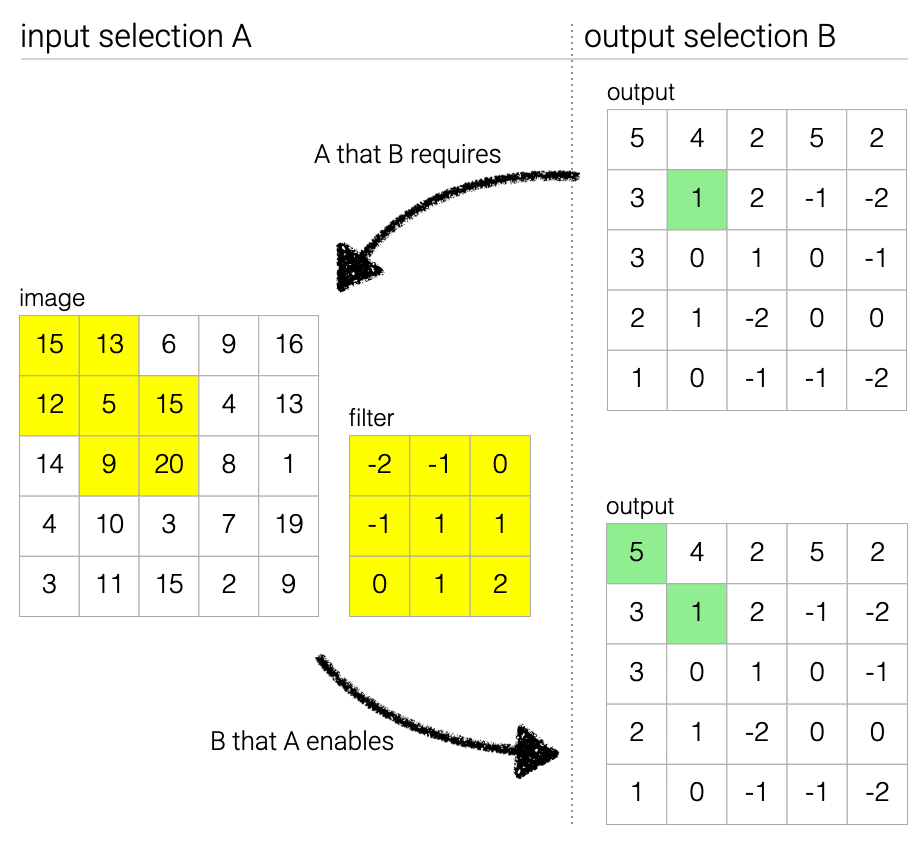
\includegraphics[scale=0.4]{fig/example/4-relations-1.png}}
      \vspace{2mm}
      \caption{Galois dependency $(\evalBwdF{T}, \evalFwdF{T})$}
      \label{fig:example:convolve-viz:galois-dependency}
   \end{subfigure}
   \begin{subfigure}{0.46\textwidth}
      {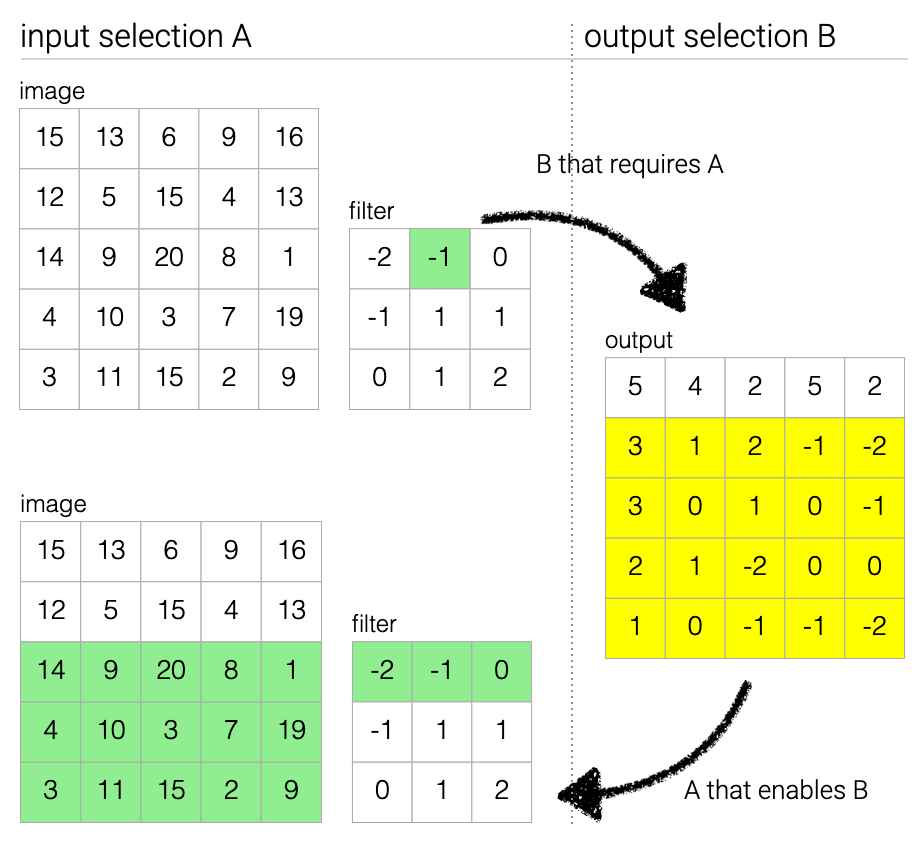
\includegraphics[scale=0.4]{fig/example/4-relations-2.png}}
      \vspace{2mm}
      \caption{De Morgan dual $(\dual{\evalFwdF{T}}, \dual{\evalBwdF{T}})$}
      \label{fig:example:convolve-viz:de-morgan-dual}
   \end{subfigure}
   \caption{Upper and lower pairs are dual; left and right pairs are adjoint}
   \label{fig:example:convolve-viz}
\end{figure}


\subsection{Relationship to Galois slicing}
\label{sec:toolkit:galois-slicing}

in the program slicing literature, dynamic analyses based on Galois connections have been developed for pure functional programs~\cite{perera12a}, functional programs with effects~\cite{ricciotti17}, and \piCalculus~\cite{perera16d}. These ``Galois slicing'' techniques have the flavour of what we need, but are unable to compute the kind of sufficiency relation we just outlined. To see the problem, we briefly outline how Galois slicing works. The idea is generalise the notion of program and value to \emph{program slices} and \emph{value slices}, program and values where some subexpressions have been replaced by hole $\hole$. A program slice ``evaluates'' to a \emph{value slice}, a value where some subvalues have been replaced by $\hole$, and dual to this, a value slice induces a (minimal) program slice. One can then extend this basic framework to focus on

The problem with this approach is that it does not readily extend to a notion of selection where the part of the output of interest is not a prefix of the output, but rather a prefix of some subtree. For example, if we consider the following program, which has the value \lstinline{(0.4, 0.6)}:

\begin{figure}
   \small
   \begin{centering}
      \begin{subfigure}{0.45\textwidth}
         {\lstinputlisting[language=Fluid,escapeinside={(*@}{@*)}]{other-src/diff-slicing-0.example}}
      \caption{Original program}
      \label{fig:example:diff-slicing:original}
      \end{subfigure}
      \begin{subfigure}{0.45\textwidth}
         {\lstinputlisting[language=Fluid,escapeinside={(*@}{@*)}]{other-src/diff-slicing-2.example}}
      \caption{Backward slice for \kw{(0.4, $\hole$)}}
      \label{fig:example:diff-slicing:subtree}
      \end{subfigure}
      \\
      \begin{subfigure}{0.45\textwidth}
         {\lstinputlisting[language=Fluid,escapeinside={(*@}{@*)}]{other-src/diff-slicing-1.example}}
      \caption{Backward slice for spine \kw{($\hole$, $\hole$)}}
      \label{fig:example:diff-slicing:spine}
      \end{subfigure}
      \begin{subfigure}{0.45\textwidth}
         {\lstinputlisting[language=Fluid,escapeinside={(*@}{@*)}]{other-src/diff-slicing-3.example}}
      \caption{Differential backward slice for \kw{(\codeSelTwo{0.4}, $\hole$)}}
      \label{fig:example:diff-slicing:differential}
      \end{subfigure}
   \end{centering}
   \vspace{-2mm}
   \caption{Differential Galois slicing selects input (blue) needed \emph{only} for selected output (green)}
   \label{fig:example:diff-slicing}
\end{figure}


\noindent Because differential slicing includes a program part if is needed \emph{only} by the selected output, in general it underapproximates the parts actually needed for the selected output. In this example, \lstinline{2} and \lstinline{3} are both needed to compute the spine containing the subtree of interest, and so the differential slice does not include them. Differential slicing based on tree prefixes is thus not a suitable technique for computing data dependencies.

Our approach does have one disadvantage vis-\'a-vis Galois slicing, namely that a program ``selection'' does not really resemble a program, but merely picks out various constants and constructors in the program involved in constructing the output selection. With Galois slicing, the program slice is a program with some holes. Although it is not executable as-is, one could (for example) imagine replacing holes by arbitrary expressions of an appropriate type, in order to recover an executable slice. It is not clear with our approach how to ``extract'' an executable slice for a particular output selection; for primitive values, one could extract the \emph{expression provenance} \cite{acar12}, which would explain how the primitive value was computed using primitive operations, but it is not easy to see how this generalises to structured outputs. Moreover there is no property that ensures the expression provenance is in some sense a projection of the semantics of the original program; \cite{field98} explore this notion of executable slice in the context of term rewriting systems, so perhaps this idea could be adapted to our core calculus and used to derive a notion of execution slice. \todo{Needs work -- perhaps move this paragraph to Related work.}
